% Section content template for individual Educative lessons
% This file contains the actual content for a specific section
% Generated from Educative API section content

% Section: Class Diagram for the Meeting Scheduler
% Section ID: 5916251618803712
% Section Slug: class-diagram-for-the-meeting-scheduler
% Generated: 2025-12-12T13:06:30.331342

Following a bottom-up approach in this lesson, we identify and design the main classes, abstract classes, and interfaces for the meeting scheduler system. Each class is tied to the requirements and use cases defined earlier, ensuring completeness, traceability, and real-world clarity.

\subsection{Components of a meeting scheduler}\label{pqOTAhq2ISYaqRQjluxHt}
\\
As mentioned, we'll design the meeting scheduler using a bottom-up approach.

\subsubsection{User}\label{BcVppnjsA2CTjDxdF51iG}
\\
The \texttt{User} class represents a person who can organize or participate in meetings. It stores personal information (such as name and email), manages their calendar, and can respond to meeting invitations.
\\
The class definition is shown below:

\begin{figure}[htbp]
 \centering
 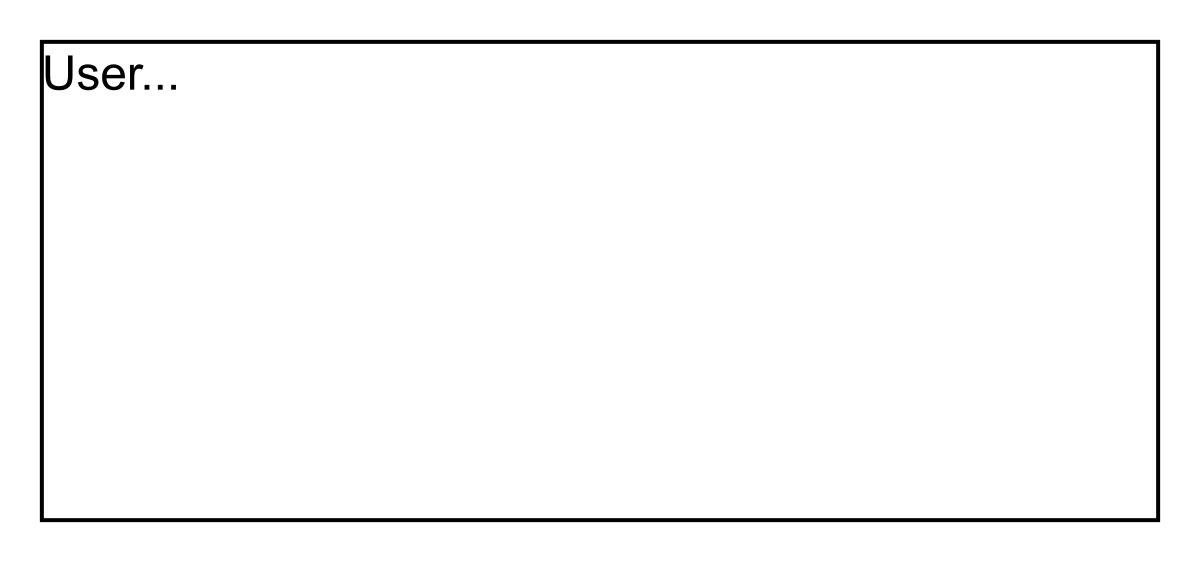
\includegraphics[width=0.5\textwidth]{Images/chapter_13/section_5916251618803712/5596583738343424.png}
 \caption{The class diagram of the User class}
\end{figure}

\textbf{R4:} When a meeting is scheduled, updated, or canceled, notifications must be sent promptly to all invited participants.
\\
\textbf{R5:} Invited participants receive meeting invites regardless of availability. The system must track each participant's invitation response status (accepted, declined, pending) within the meeting record.
\\
\textbf{R6:} Every user must have access to a personal calendar to view, schedule, or cancel meetings, and to track all meeting invitations and responses.

\subsubsection{Interval}\label{twppWpSiToBi0EzDEwEhu}
\\
The \texttt{Interval} class contains the start time and end time of a meeting. The visual representation of the \texttt{Interval} class is as follows:

\begin{figure}[htbp]
 \centering
 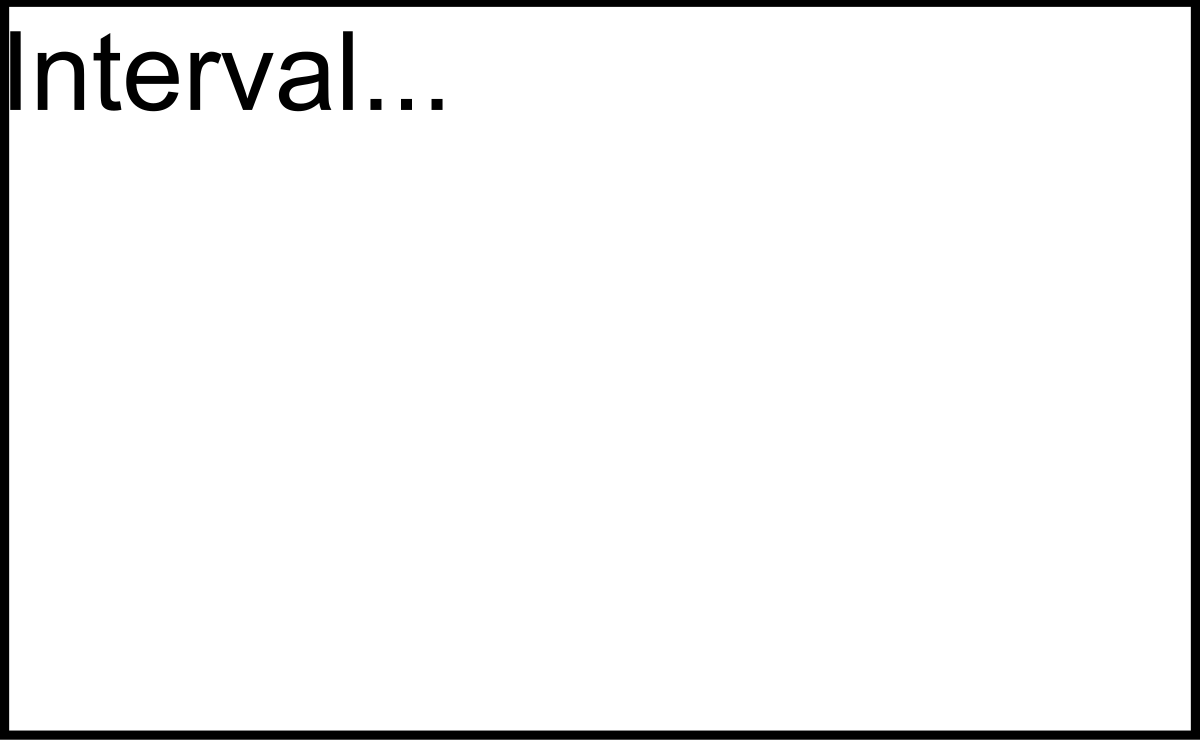
\includegraphics[width=0.5\textwidth]{Images/chapter_13/section_5916251618803712/4766614941859840.png}
 \caption{The class diagram of the Interval class}
\end{figure}

\textbf{R3:} Meeting rooms can be booked for specific time intervals, provided they are available and not already reserved for overlapping times.

\subsubsection{MeetingRoom}\label{hFzZET3RCxEY7x8Pc--ri-1}
\\
The \texttt{MeetingRoom} class contains the details of any particular room, such as its capacity and status, to identify whether it is currently available. It also contains a list of intervals to track when the room is booked for a meeting.
\\
The class diagram of the \texttt{MeetingRoom} class is provided below:

\begin{figure}[htbp]
 \centering
 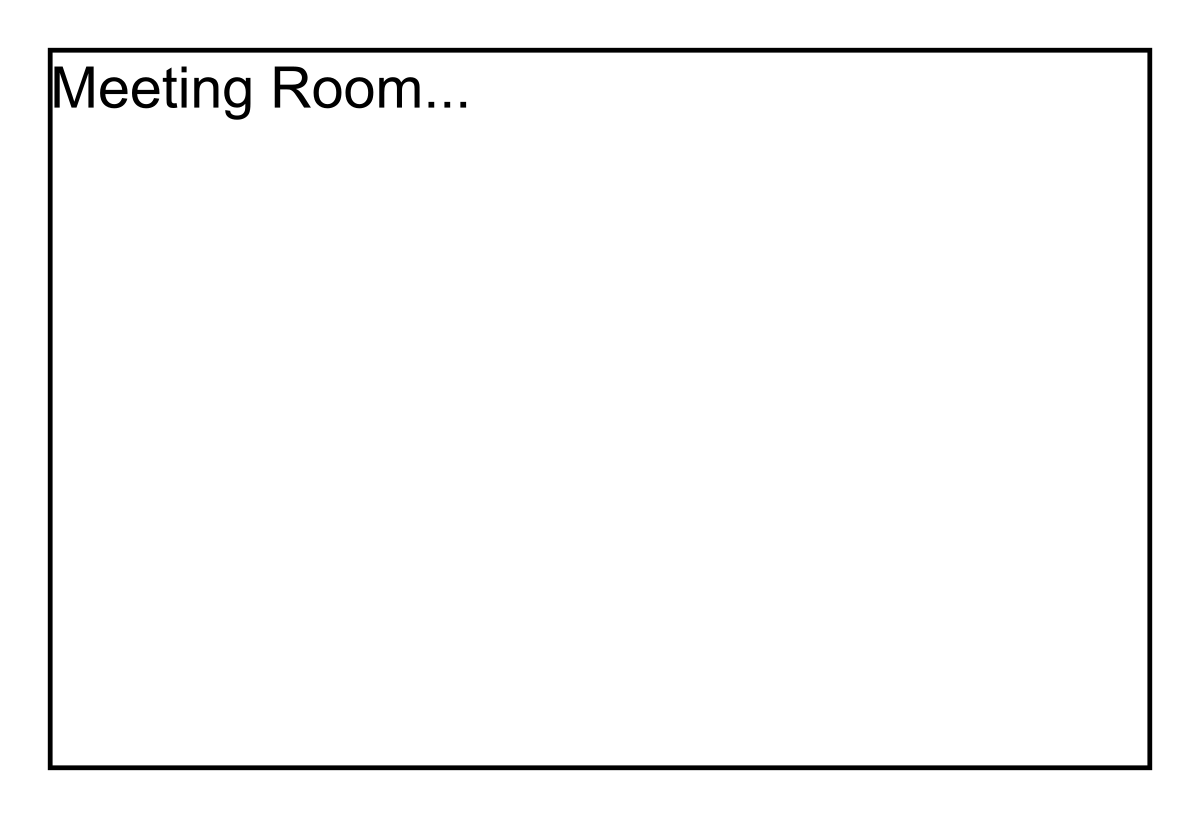
\includegraphics[width=0.5\textwidth]{Images/chapter_13/section_5916251618803712/6425010141790208.png}
 \caption{The class diagram of the MeetingRoom class}
\end{figure}

\textbf{R1:} The system must support a configurable number of meeting rooms, allowing organizations to add or manage rooms as needed.
\\
\textbf{R2:} Each meeting room must have a defined capacity, ensuring only meetings within the room's limits can be scheduled.
\\
\textbf{R3:} Meeting rooms can be booked for specific time intervals, provided they are available and not already reserved for overlapping times.
\\
\textbf{R8:} The system must handle booking conflicts and overlapping meetings, providing clear feedback if a room or participant is already booked for the requested time.

\subsubsection{Meeting}\label{swkpSyiAJ-FnCDXknDch3}
\\
The \texttt{Meeting} class holds all details about a meeting, including the participants, their RSVP statuses, scheduled time, room, and subject.
\\
The class diagram of the \texttt{Meeting} class is provided below:

\begin{figure}[htbp]
 \centering
 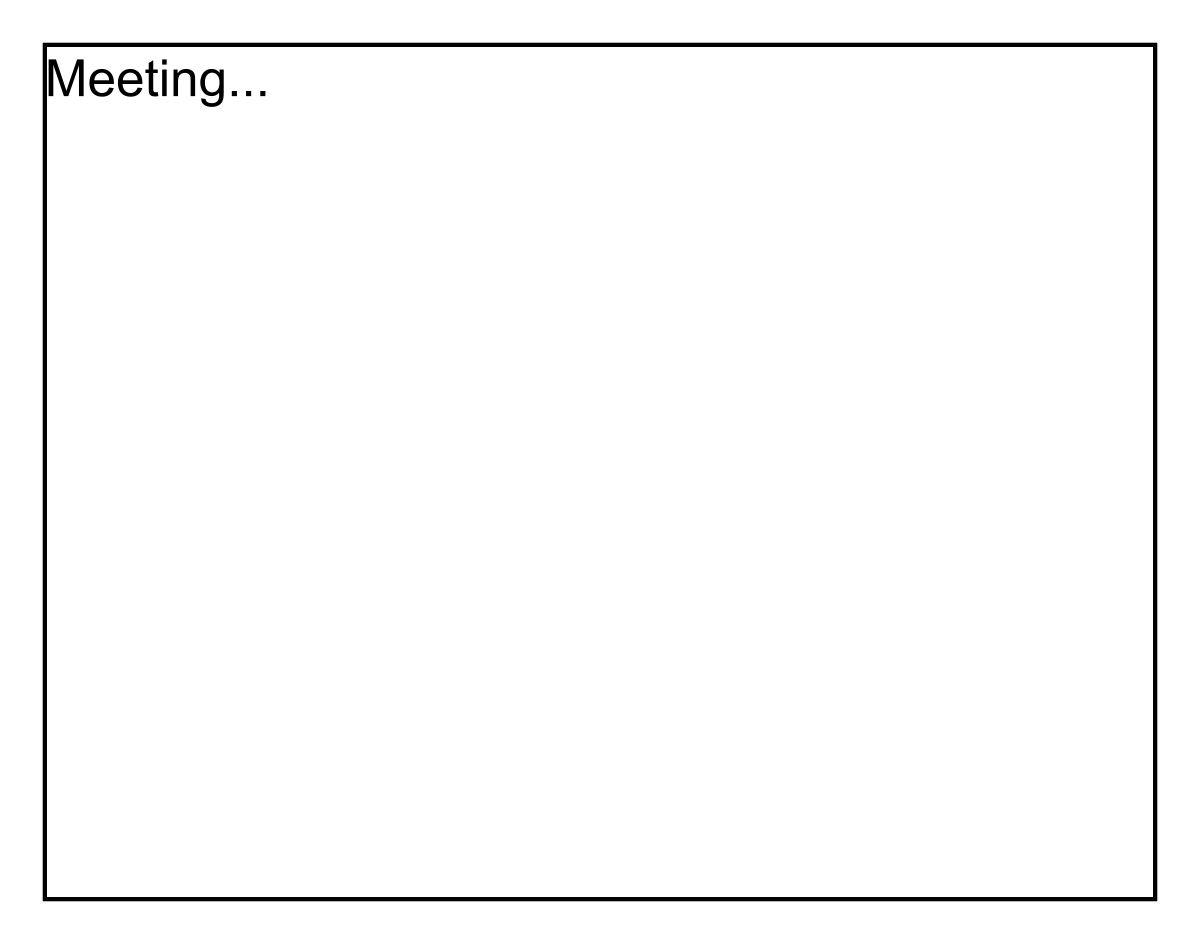
\includegraphics[width=0.5\textwidth]{Images/chapter_13/section_5916251618803712/6102814370430976.png}
 \caption{The class diagram of the Meeting class}
\end{figure}

\textbf{R5:} Invited participants receive meeting invites regardless of their current availability. The system must track each participant's invitation response status (accepted, declined, pending) within the meeting record.
\\
\textbf{R7:} The organizer must be able to add or remove participants after a meeting has been scheduled, and appropriate notifications must be sent for any changes.
\\
\textbf{R9:} Meeting details (such as title, agenda, room, time, and participant list) should be editable by the organizer, with all updates triggering notifications.
\\
\textbf{R10:} The system should support meeting cancellations by the organizer or authorized participants and notify all invitees of the cancellation.

\subsubsection{Calendar}\label{hFzZET3RCxEY7x8Pc--ri-2}
\\
The \texttt{Calendar} class tracks all user meetings and allows adding or removing meetings based on user actions or meeting status changes.
\\
The class definition is provided below:

\begin{figure}[htbp]
 \centering
 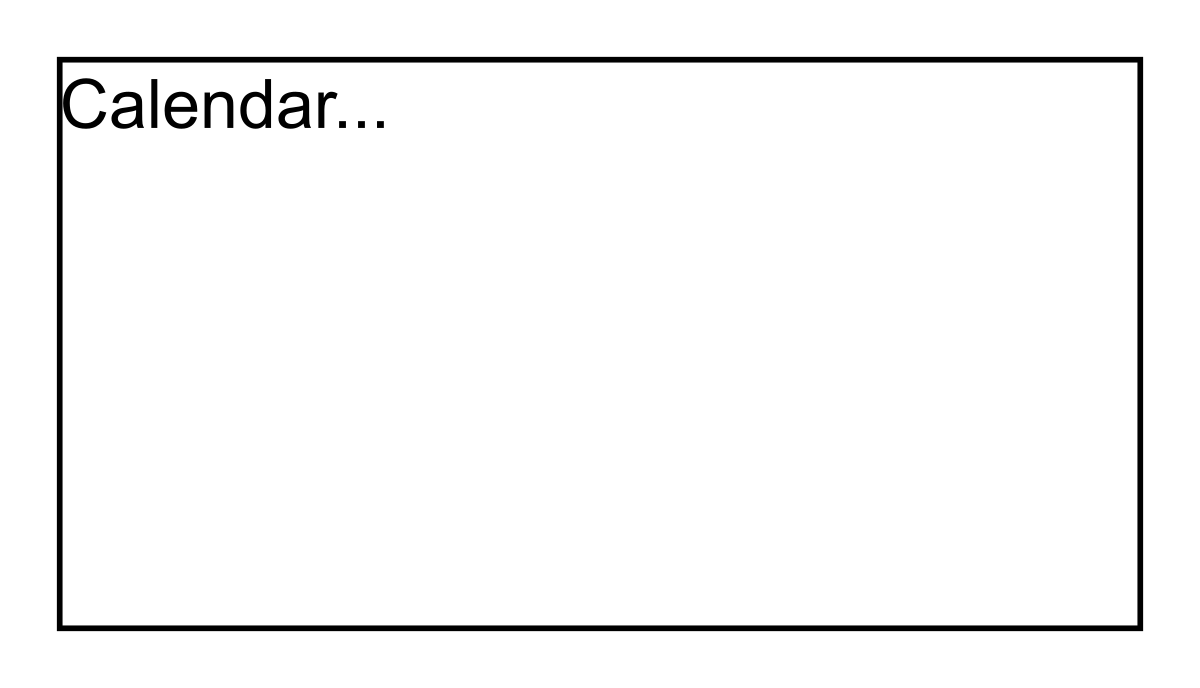
\includegraphics[width=0.5\textwidth]{Images/chapter_13/section_5916251618803712/5970053240324096.png}
 \caption{The class diagram of the Calendar class}
\end{figure}

\textbf{R6:} Every user must have access to a personal calendar to view, schedule, or cancel meetings, and to track all meeting invitations and responses.
\\
\textbf{R11:} If a participant declines an invite or withdraws from a meeting, the meeting must be removed from their calendar, and their response status updated in the meeting record. The meeting should remain active for other participants unless canceled by the organizer.

\subsubsection{MeetingScheduler}\label{UhZSkr_T-ji6-tul56ch2-1}
\\
The \texttt{MeetingScheduler} class coordinates the overall scheduling process. It manages the list of meeting rooms, schedules and cancels meetings, checks room availability, books and releases rooms, and triggers notifications.
\\
The visual representation of the \texttt{MeetingScheduler} class is provided below:

\begin{figure}[htbp]
 \centering
 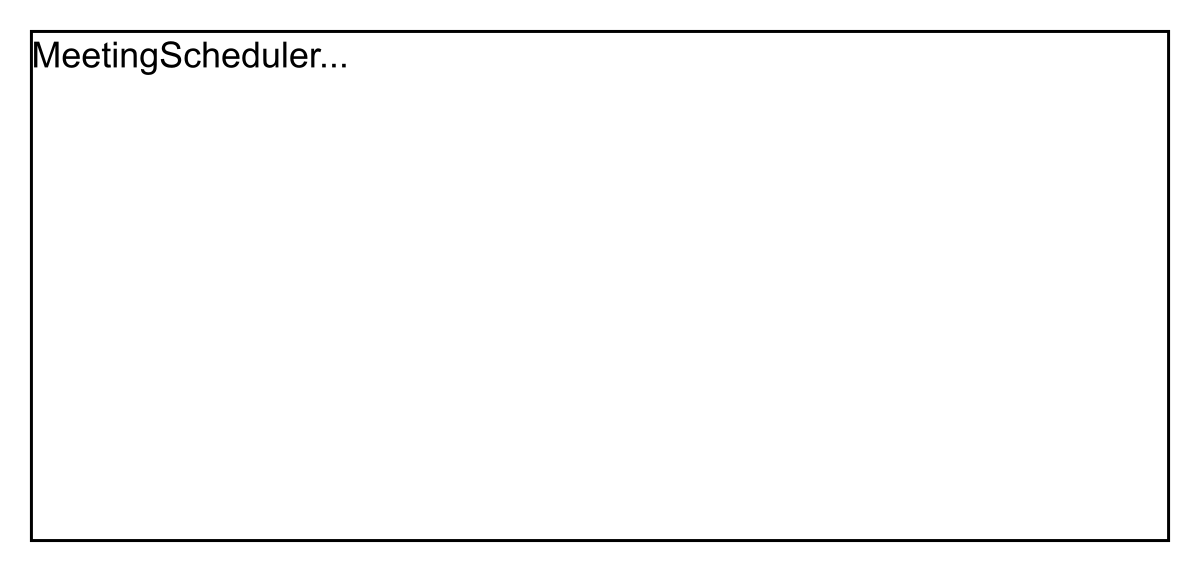
\includegraphics[width=0.5\textwidth]{Images/chapter_13/section_5916251618803712/5333053898358784.png}
 \caption{Class diagram of the MeetingScheduler class}
\end{figure}

\textbf{R1:} The system must support a configurable number of meeting rooms, allowing organizations to add or manage rooms as needed.
\\
\textbf{R2:} Each meeting room must have a defined capacity, ensuring only meetings within the room's limits can be scheduled.
\\
\textbf{R3:} Meeting rooms can be booked for specific time intervals, provided they are available and not already reserved for overlapping times.
\\
\textbf{R7:} The organizer must be able to add or remove participants after a meeting has been scheduled, and appropriate notifications must be sent for any changes.
\\
\textbf{R8:} The system must handle booking conflicts and overlapping meetings, providing clear feedback if a room or participant is already booked for the requested time.
\\
\textbf{R10:} The system should support meeting cancellations by the organizer or authorized participants and notify all invitees of the cancellation.
\\
\textbf{R12:} Any updates to a meeting (e.g., time, room, or participants) should automatically update all relevant calendars and trigger notifications.

\subsubsection{Notification}\label{UhZSkr_T-ji6-tul56ch2-2}
\\
The \texttt{Notification} class will send a notification for an invitation to a user regarding any new meeting. It will also send a cancellation notification to a user in case any meeting gets canceled or is postponed.
\\
The UML representation of the class is shown below:

\begin{figure}[htbp]
 \centering
 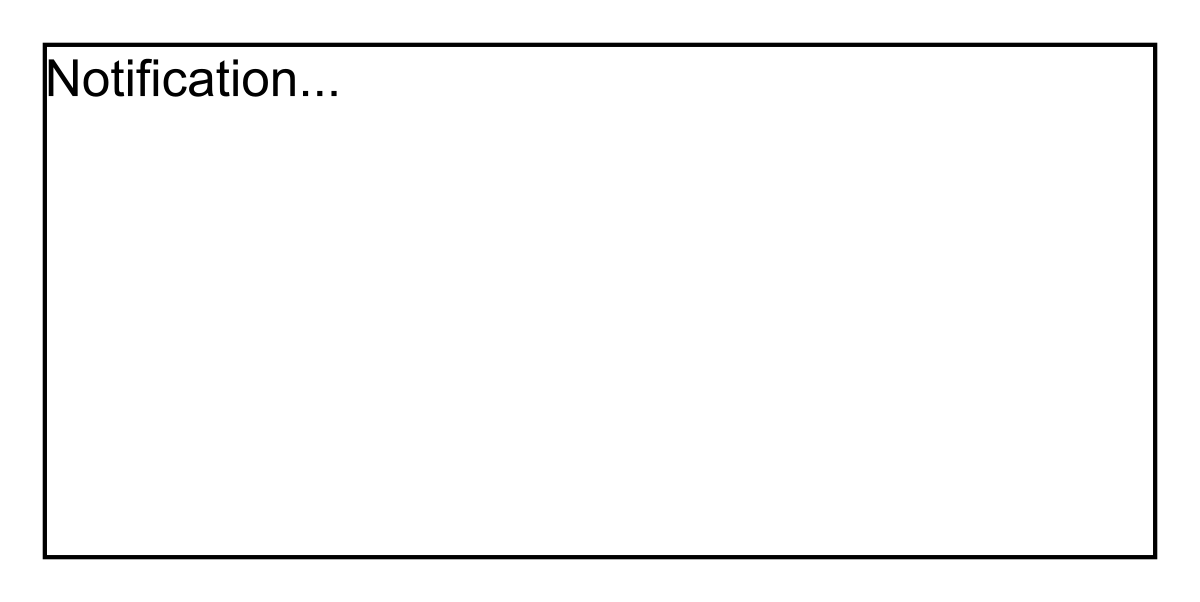
\includegraphics[width=0.5\textwidth]{Images/chapter_13/section_5916251618803712/6204042924392448.png}
 \caption{The class diagram of the Notification class}
\end{figure}

\textbf{R4:} A notification should be sent to everyone invited to the meeting.

\subsubsection{Enumerations}\label{8b0Cn6cUToTmFIJd3JyDR}
\\
Enumeration is generally a data type in which only a specific set of constants can be stored. Following is the list of enumerations required in the meeting scheduler system:
\\
RSVPStatus\ (Enum): Tracks the current status of each participant's response to a meeting invite.

\begin{figure}[htbp]
 \centering
 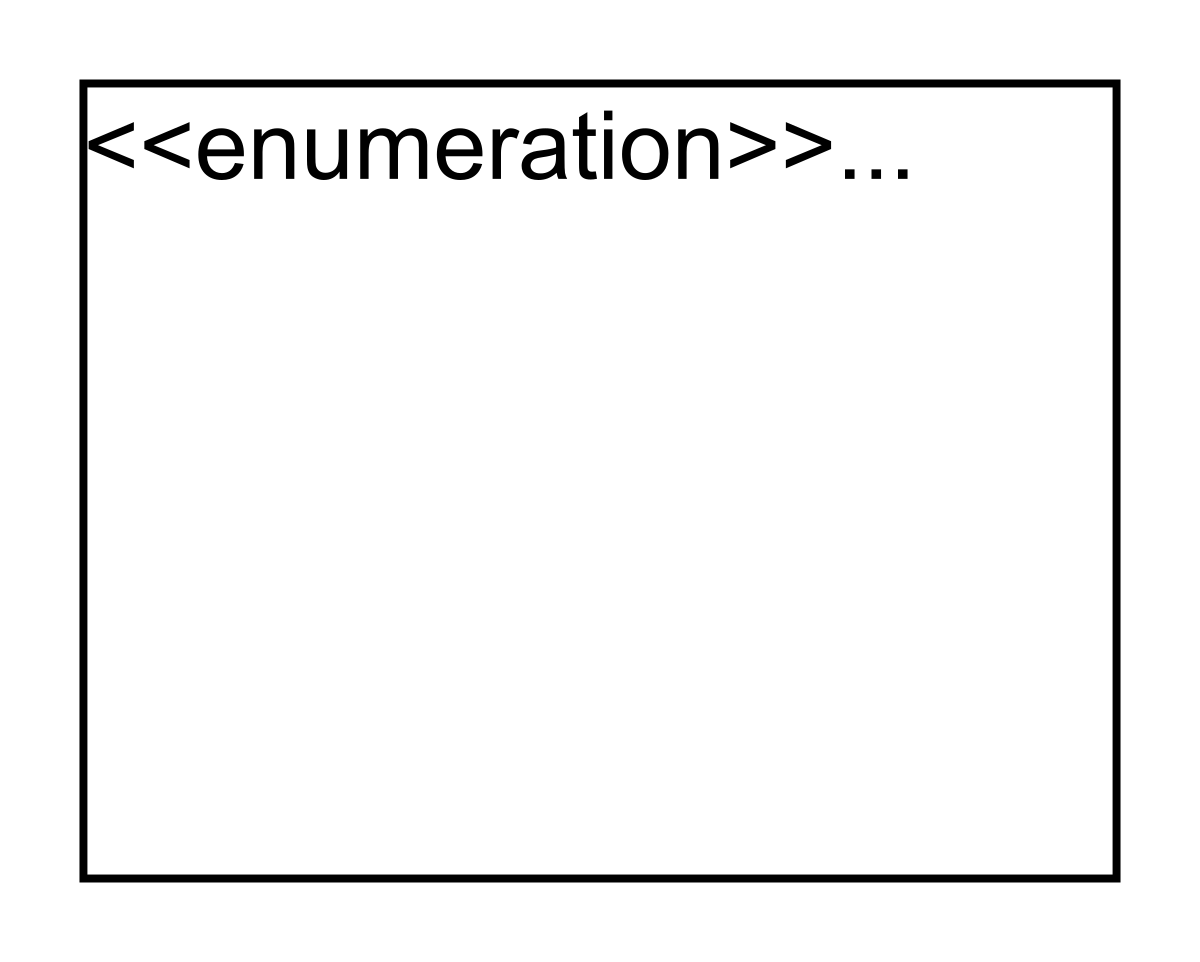
\includegraphics[width=0.5\textwidth]{Images/chapter_13/section_5916251618803712/4823238486917120.png}
 
\end{figure}

\textbf{R5:} Invited participants receive meeting invites regardless of their current availability. The system must track each participant's invitation response status (accepted, declined, pending) within the meeting record.

\subsection{Relationship between the classes}\label{spPUwOm3kRzPiqkKehu98-2}
\\
Now, we'll discuss the relationships between the above-mentioned classes in the meeting scheduler.

\subsubsection{Association}\label{YqAMMVA2tW4kkut5VHdxz}
\\
The class diagram has the following association relationships:

\begin{itemize}
\item
\protect\phantomsection\label{T3igafhO6phivlAtVaC-S}
\texttt{User} and \texttt{Meeting}:

\begin{itemize}
\item
Each \texttt{User} can be an organizer or a participant in multiple \texttt{Meeting} instances. Each
\texttt{Meeting} maintains a mapping (Map\textless{User,\ RSVPStatus\textgreater{}}) of all its participants and their current invitation status.
\end{itemize}
\item
\protect\phantomsection\label{OEW0-KhPcOBRX4P6kf3XM}
\texttt{Meeting} and \texttt{MeetingRoom}:

\begin{itemize}
\item
Each \texttt{Meeting} is assigned to a single \texttt{MeetingRoom}. Each \texttt{MeetingRoom} can host many meetings (at different intervals).
\end{itemize}
\item
\protect\phantomsection\label{sb2ow6AKDlTR9AkP4-qWD}
\texttt{Notification} and \texttt{User}:

\begin{itemize}
\item
\texttt{Notification} objects are sent to users whenever a meeting is scheduled, updated, or canceled.
\end{itemize}
\end{itemize}

\begin{figure}[htbp]
 \centering
 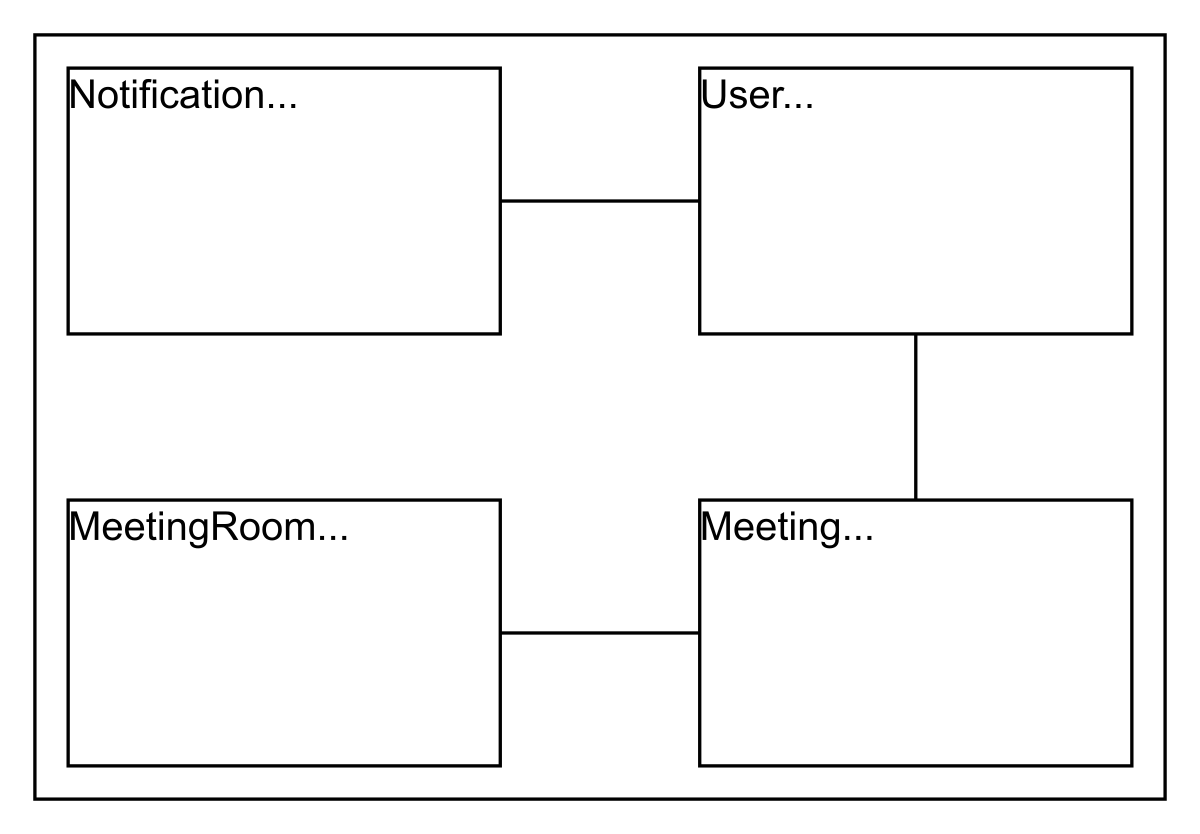
\includegraphics[width=0.5\textwidth]{Images/chapter_13/section_5916251618803712/5225130354409472.png}
 \caption{The association relationship between classes}
\end{figure}

\subsubsection{Composition}\label{spPUwOm3kRzPiqkKehu98-3}
\\
The class diagram has the following composition relationships:

\begin{itemize}
\item
\protect\phantomsection\label{p5XyIM_nB2zclNMpkYrXs}
\texttt{User} and \texttt{Calendar}:

\begin{itemize}
\item
Each \texttt{User} composes exactly one \texttt{Calendar}. If the user is deleted, their calendar is deleted as well.
\end{itemize}
\item
\protect\phantomsection\label{xFbDkR13jHciGOqviUe2a}
\texttt{Calendar} and \texttt{Meeting}:

\begin{itemize}
\item
Each \texttt{Calendar} comprises multiple \texttt{Meeting} objects (as the user accepts or schedules meetings).
\end{itemize}
\item
\protect\phantomsection\label{7vSHmAi8ghmeKy6T7AcDP}
\texttt{Meeting} and \texttt{Interval}:

\begin{itemize}
\item
Each \texttt{Meeting} is scheduled for a single \texttt{Interval}. Each \texttt{MeetingRoom} keeps a list of all booked \texttt{Intervals}.
\end{itemize}
\end{itemize}

\begin{figure}[htbp]
 \centering
 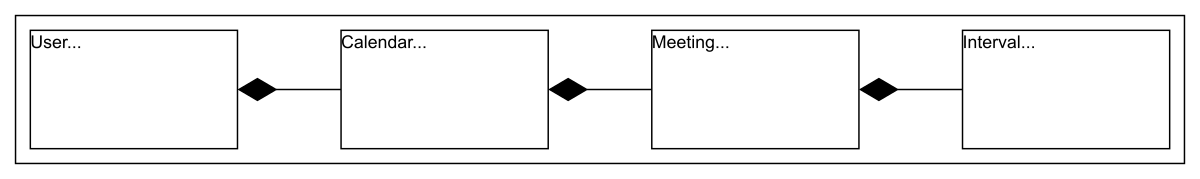
\includegraphics[width=0.5\textwidth]{Images/chapter_13/section_5916251618803712/5879583277449216.png}
 \caption{The composition relationship between classes}
\end{figure}

\subsubsection{Aggregation}\label{spPUwOm3kRzPiqkKehu98-4}
\\
The class diagram has the following aggregation relationships:

\begin{itemize}
\item
\protect\phantomsection\label{b_87u-5nSpfYjxU909l3B}
\texttt{MeetingScheduler} and \texttt{MeetingRoom}:

\begin{itemize}
\item
The \texttt{MeetingScheduler} aggregates all available \texttt{MeetingRoom} instances and manages their booking and release.
\end{itemize}
\item
\protect\phantomsection\label{clTjrX-oPf1yWIpTZW1dV}
\texttt{MeetingScheduler} and \texttt{Meeting}:

\begin{itemize}
\item
The \texttt{MeetingScheduler} aggregates and manages all scheduled \texttt{Meeting} instances for the organization.
\end{itemize}
\item
\protect\phantomsection\label{YvPjhJdZPvY8-cY5XXB-B}
\texttt{MeetingRoom} and \texttt{Interval}:

\begin{itemize}
\item
Each \texttt{MeetingRoom} aggregates a collection of booked \texttt{Interval} s, representing its occupied time slots.
\end{itemize}
\end{itemize}

\begin{figure}[htbp]
 \centering
 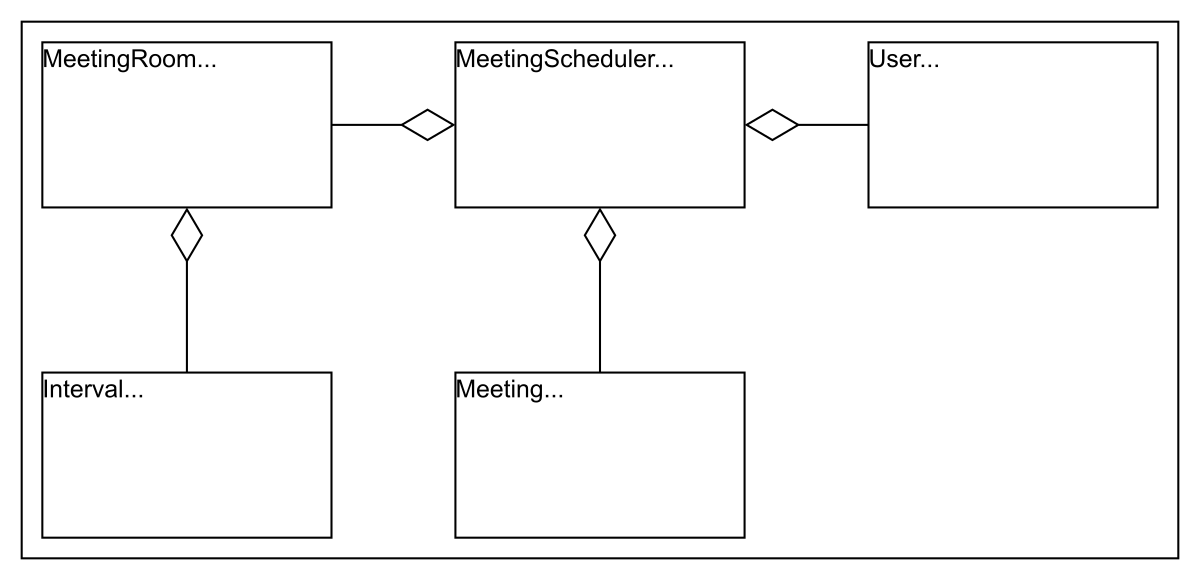
\includegraphics[width=0.5\textwidth]{Images/chapter_13/section_5916251618803712/6695567311634432.png}
 \caption{The aggregation relationship between classes}
\end{figure}

\subsection{Class diagram of the meeting scheduler}\label{spPUwOm3kRzPiqkKehu98-5}
\\
This section outlines the multiplicity (cardinality) relationships between the main classes in our meeting scheduler. For each relationship, we explain the allowed number of instances on each side and the real-world or design rationale behind the connection. Understanding these relationships is key to modeling how different entities interact and collaborate to support key workflows in the system.

\begin{center}
\begin{tabular}{|p{0.20\linewidth}|p{0.20\linewidth}|p{0.15\linewidth}|p{0.38\linewidth}|}
\hline
\textbf{Source} & \textbf{Target} & \textbf{Multiplicity} & \textbf{Reason} \\
\hline

User & Calendar & 1--1 &
Each user has exactly one calendar, and each calendar belongs to one user. \\
\hline

User & Meeting & 1--0..* &
A user can organize or participate in multiple meetings (including zero). \\
\hline

MeetingRoom & Meeting & 1--0..* &
A room can host zero or more meetings over time. \\
\hline

Meeting & Interval & 1--1 &
Each meeting occupies exactly one time interval (start and end). \\
\hline

MeetingRoom & Interval & 1--0..* &
Each room tracks all intervals it is booked for. \\
\hline

Calendar & Meeting & 1--0..* &
A user’s calendar contains all meetings associated with that user. \\
\hline

MeetingScheduler & MeetingRoom & 1--1..* &
The scheduler manages one or more meeting rooms. \\
\hline

MeetingScheduler & Meeting & 1--1..* &
The scheduler manages zero or more meetings. \\
\hline

User & MeetingScheduler & 1--0..* &
The scheduler can manage one or more users. \\
\hline

\end{tabular}
\end{center}


Here's the complete class diagram for the meeting scheduler:

\begin{figure}[htbp]
 \centering
 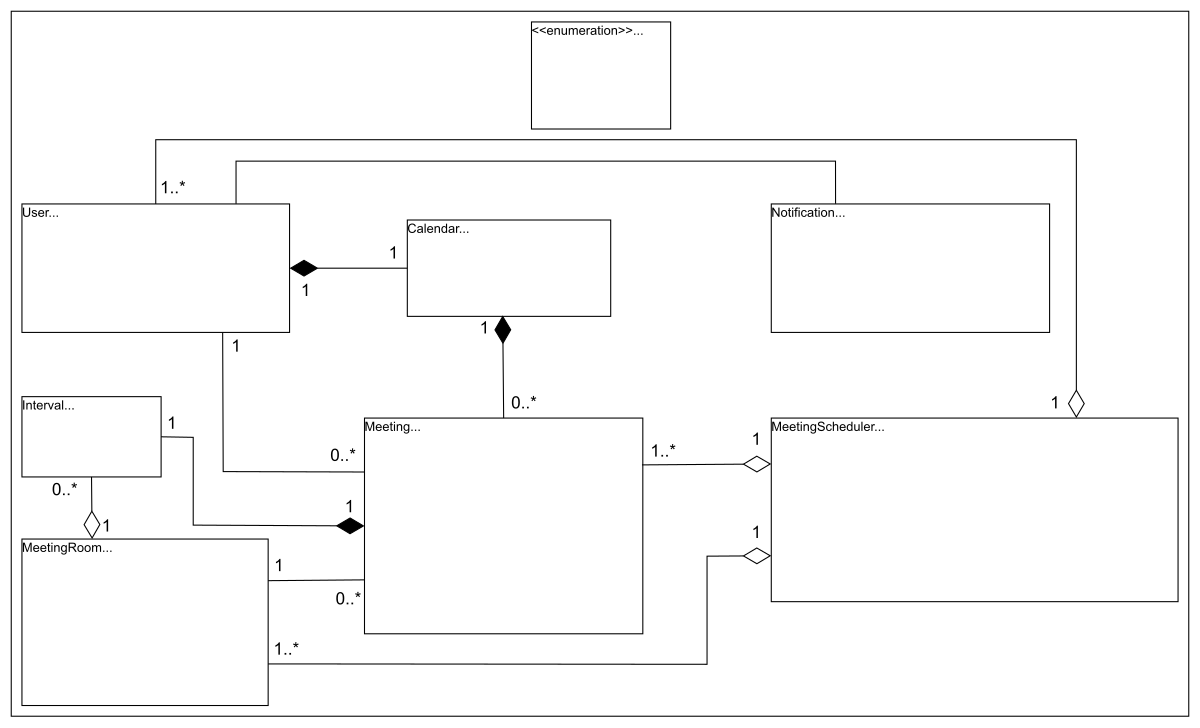
\includegraphics[width=0.5\textwidth]{Images/chapter_13/section_5916251618803712/5219881669492736.png}
 \caption{The class diagram of the meeting scheduler}
\end{figure}

\subsection{Design pattern}\label{W336gs5Ox_T0Zw3xsSS02}
\\
Several classic object-oriented design patterns are applied in the meeting scheduler system to ensure a robust, scalable, and maintainable design.

\begin{itemize}
\item
\protect\phantomsection\label{yM1gTHOCYWPhsZuVkKPD4}
\textbf{Singleton pattern:} The core scheduling functionality is centralized in the \texttt{MeetingScheduler} class, ensuring that only one active instance is responsible for managing all meetings, rooms, and scheduling operations across the system. This is achieved using the Singleton pattern, which restricts the instantiation of the scheduler to a single, globally accessible object.
\item
\protect\phantomsection\label{G8yDNCn4N5fLD9hT5QSiA}
\textbf{Observer pattern:} For user notifications, the system employs the Observer pattern. When a meeting is scheduled, updated, or canceled, all relevant users (participants or organizers) are notified automatically. This decouples the notification logic from the rest of the business workflow and ensures users always receive timely updates.
\end{itemize}

\subsection{AI-powered trainer}\label{GuDntinc_KKHiovtvBxA8}
\\
At this stage, everything should be clear. If you encounter any confusion or ambiguity, feel free to utilize the interactive AI-enabled widget below to seek clarification. This tool is designed to assist you in strengthening your understanding of the concepts.

\begin{figure}[htbp]
 \centering
 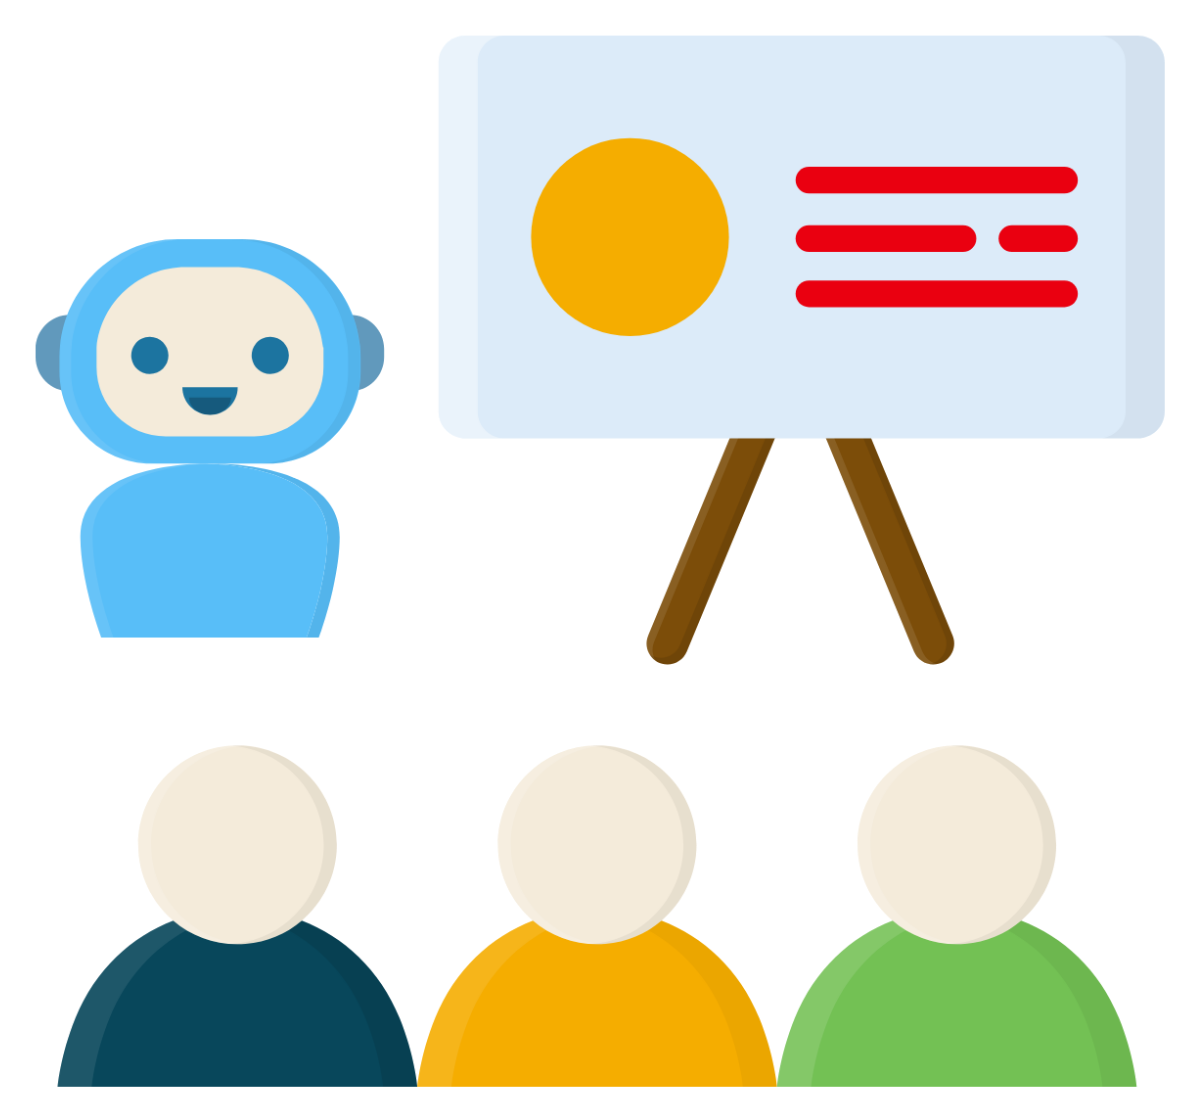
\includegraphics[width=0.15\textwidth]{Images/chapter_13/section_5916251618803712/5181938951127040.png}
 
\end{figure}

We have completed the class diagram of the meeting scheduler according to the requirements. In the next lesson, let's design the sequence diagram of the meeting scheduler.

% End of section content